%%%%%%%%%%%%%%%%%%%%%%%%%%%%%%%%%%%%%%%%%
% Short Sectioned Assignment
% LaTeX Template
% Version 1.0 (5/5/12)
%
% This template has been downloaded from:
% http://www.LaTeXTemplates.com
%
% Original author:
% Frits Wenneker (http://www.howtotex.com)
%
% License:
% CC BY-NC-SA 3.0 (http://creativecommons.org/licenses/by-nc-sa/3.0/)
%
%%%%%%%%%%%%%%%%%%%%%%%%%%%%%%%%%%%%%%%%%

%----------------------------------------------------------------------------------------
%	PACKAGES AND OTHER DOCUMENT CONFIGURATIONS
%----------------------------------------------------------------------------------------

\documentclass[paper=a4, fontsize=11pt]{article} % A4 paper and 11pt font size

\usepackage{float}
%\usepackage[backend=bibtex,style=verbose-trad2]{biblatex}
% table related packages
\usepackage{multirow} % multirow of table
\usepackage{array}
\usepackage{tabulary}
\newcolumntype{K}[1]{>{\centering\arraybackslash}p{#1}}

\usepackage{algorithm} % two are used to demonstrate algorithm
\usepackage{fullpage}

\usepackage[toc,page]{appendix} % appendices
\usepackage[T1]{fontenc} % Use 8-bit encoding that has 256 glyphs
\usepackage{fourier} % Use the Adobe Utopia font for the document - comment this line to return to the LaTeX default
\usepackage[english]{babel} % English language/hyphenation
\usepackage{amsmath,amsfonts,amsthm,amssymb} % Math packages
\usepackage{bbm} % for characteristic function
\usepackage{algpseudocode}
\usepackage{algorithm} % two are used to demonstrate algorithm
\usepackage{graphicx} % for adding graphics
\usepackage{lipsum} % Used for inserting dummy 'Lorem ipsum' text into the template
\usepackage{sectsty} % Allows customizing section commands
%\usepackage{natbib}

\usepackage{fancyhdr} % Custom headers and footers
\pagestyle{fancyplain} % Makes all pages in the document conform to the custom headers and footers
\fancyhead{} % No page header - if you want one, create it in the same way as the footers below
\fancyfoot[L]{} % Empty left footer
\fancyfoot[C]{} % Empty center footer
\fancyfoot[R]{\thepage} % Page numbering for right footer
\renewcommand{\headrulewidth}{0pt} % Remove header underlines
\renewcommand{\footrulewidth}{0pt} % Remove footer underlines
\setlength{\headheight}{13.6pt} % Customize the height of the header

\numberwithin{equation}{section} % Number equations within sections (i.e. 1.1, 1.2, 2.1, 2.2 instead of 1, 2, 3, 4)
\numberwithin{table}{section} % Number tables within sections (i.e. 1.1, 1.2, 2.1, 2.2 instead of 1, 2, 3, 4)

\setlength\parindent{0pt} % Removes all indentation from paragraphs - comment this line for an assignment with lots of text

% this part is for inserting Python code:
% Default fixed font does not support bold face
\DeclareFixedFont{\ttb}{T1}{txtt}{bx}{n}{12} % for bold
\DeclareFixedFont{\ttm}{T1}{txtt}{m}{n}{12}  % for normal

% Custom colors
\usepackage{color}
\definecolor{deepblue}{rgb}{0,0,0.5}
\definecolor{deepred}{rgb}{0.6,0,0}
\definecolor{deepgreen}{rgb}{0,0.5,0}

\usepackage{listings}

% Python style for highlighting
\newcommand\pythonstyle{\lstset{
language=Python,
basicstyle=\ttm,
otherkeywords={self},             % Add keywords here
keywordstyle=\ttb\color{deepblue},
emph={MyClass,__init__},          % Custom highlighting
emphstyle=\ttb\color{deepred},    % Custom highlighting style
stringstyle=\color{deepgreen},
frame=tb,                         % Any extra options here
showstringspaces=false            % 
}}

\usepackage[utf8]{inputenc}
\usepackage[english]{babel}
\usepackage{subfig}
 
% Python environment
\lstnewenvironment{python}[1][]
{
\pythonstyle
\lstset{#1}
}
{}

% Python for external files
\newcommand\pythonexternal[2][]{{
\pythonstyle
\lstinputlisting[#1]{#2}}}

\setlength{\parindent}{4em}
\setlength{\parskip}{1em}
%\renewcommand{\baselinestretch}{2.0}

\usepackage{epstopdf}
\epstopdfDeclareGraphicsRule{.tif}{png}{.png}{convert #1 \OutputFile}
\AppendGraphicsExtensions{.tif}

%----------------------------------------------------------------------------------------
%	TITLE SECTION
%----------------------------------------------------------------------------------------

\newcommand{\horrule}[1]{\rule{\linewidth}{#1}} % Create horizontal rule command with 1 argument of height

\title{	
\normalfont \normalsize 
\horrule{0.5pt} \\[0.4cm] % Thin top horizontal rule
\textsc{\normalsize BME 513. Project Report Part II } \\
\huge Switching Behavior of Izhikevich Model \\ % The assignment title
\huge $\:$ \\
\large Application of Izhikevich model for working memory in neural network \\ % subtitle of the assignment
\horrule{2pt} \\[0.5cm] % Thick bottom horizontal rule
}

\author{Jaehong Yoon$^a$ Zhongxi Li$^a$\\
\normalsize $^a$ Duke University, Biomedical Engineering\\ [25pt] % Your university, school and/or department name(s)
} % Your name

\date{\normalsize\today} % Today's date or a custom date

\DeclareMathOperator*{\argminA}{arg\,min} % Jan Hlavacek
\newcommand{\cs}[1]{\texttt{\symbol{`\\}#1}}

%\newcommand{\newproblem}[1]{\newpage\subsection*{#1}}
\newcommand{\includeCode}[1]{\VerbatimInput[fontsize=\small,fontshape=rm]{#1}}
\newcommand\Myperm[2][^n]{\prescript{#1\mkern-2.5mu}{}P_{#2}}
\newcommand\tab[1][1cm]{\hspace*{#1}}

\begin{document}

\maketitle % Print the title

%----------------------------------------------------------------------------------------
%	Problem 1
%----------------------------------------------------------------------------------------

\section*{Topic} 

The team will utilize the linear analysis method for materializing working memory on biologically inspired neural network. As Nakahara and Doya ~\cite{nakahara1998near} have demonstrated, the sigmoidal neuron model near saddle node bifurcation maintain the high firing state for a period before dropping to quiescent state. As the working memory should both hold the information but also be able to transit to new state when a new information is gathered, such behavior is useful for dynamics of working memory. The persistance of firing rate for a given period can be thought of as information stored in a neuron before either new information is given (a new external current) or until the memory retaining period is over.

However, the paper does rely on simple sigmoid model which is not a phenomenological model as FitzHugh-Nagumo model~\cite{Izhikevich:2006} or Hindmarsh-Rose model~\cite{hindmarsh1984model} nor it is a common activation function for the spiking neural network~\cite{maass1997networks}. Therefore, even if the idea of the paper brings inspiration of how bifurcation in single neuron level can be used to analyze the expected behavior of the whole neural network, the intrinsic limit exist. The team will explore the use of same technique on neural network based on Izhikevich model~\cite{izhikevich2003simple} which is both computationally inexpensive and phenomenologically extra-ordinary. With simply twitching the 4 parameters of Izhikevich model, one can generate the firing pattern of spiking, bursting, chattering and even thalamo-cortical neuron. The value of parameter 'a' and 'b' of Izhikevich model in bifurcation node with other parameters being fixed (c = -65, d = 2) will be explored to observe which combination of 'a' and 'b' will be optimal for utilizing working memory. The result will be compared with both values restored from evolutionary program as in  Nakahara and Doya~\cite{nakahara1998near} and with mapping model of Izhikevich model~\cite{moehlis2008dynamical}. Finally, the values of 'a' and 'b' retrieved from the analysis will be applied to biologically inspired neural network as an demonstration~\cite{braitenberg1986vehicles, french2005introducing}.

\begin{figure}[H]
\centering
  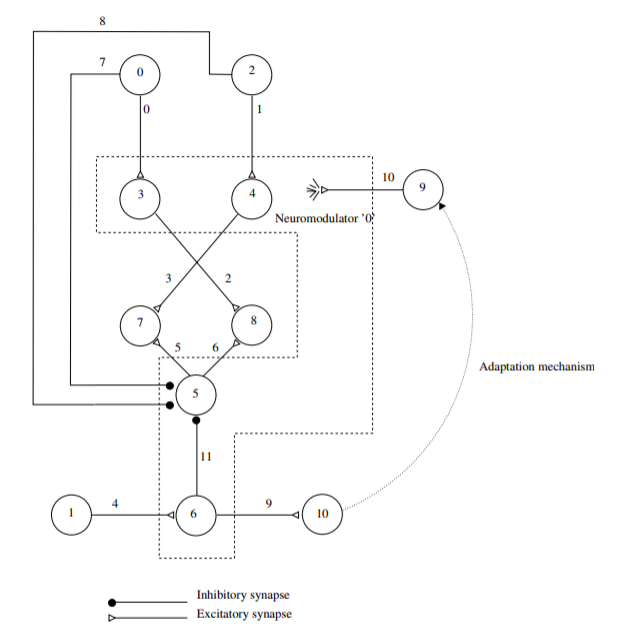
\includegraphics[width = 100mm, scale = 0.8]{./fig/Braienteg_vehicle.png}
  \caption{The sample of Brainteg vehicle neural network for demonstration of working memory. The figure was taken from Fig. 4. of French et al~\cite{french2005introducing}.}
  \label{fig1}
\end{figure}

\section*{Articles of Interest} 

The main idea of the project was inspired by Nakahara and Doya~\cite{nakahara1998near}. The model for spiking neural network and analysis of bifurcation in neuron level will be based on Izhikevich model~\cite{izhikevich2003simple, moehlis2008dynamical}.

\section*{Outline of Presentation}

As aformentioned, the team will concentrate first on the analysis of bifurcation types and the firing behavior near the bifurcations to demonstrate the expected optimal values of parameter 'a' and 'b' for working memory. As working memory should both persist for a certain period but also be able to transit to another state when new information is given, the evolutionary programming will optimize the parameter 'a' and 'b' which enables the neuron to immediately transit to high firing rate and retain the state for awhle and drop to quiescent state when new information is given. That is, as in figure~\ref{fig2}, if the time range is divided into three section where 

\begin{itemize}
\item \textbf{A}: Before external current (information) given
\item \textbf{B}: After first external current is given and before second external current was given.
\item \textbf{C}: After third external current was given
\end{itemize}

The constraint of optimization will be $ \argminA_{a, b} \frac{\textrm{average firing rate in}(A)}{\textrm{average firing rate in}(B)} \frac{\textrm{average firing rate in}(C)}{\textrm{average firing rate in}(B)}$. The result will be compared with the expected (a, b) values from bifurcation node analysis of Izhikevich model~\cite{izhikevich2003simple, moehlis2008dynamical}. Finally, the both values will be used to build Braitenberg Vehicle to demonstrate that working memory was implemented~\cite{braitenberg1986vehicles, french2005introducing}.

\begin{figure}[H]
\centering
  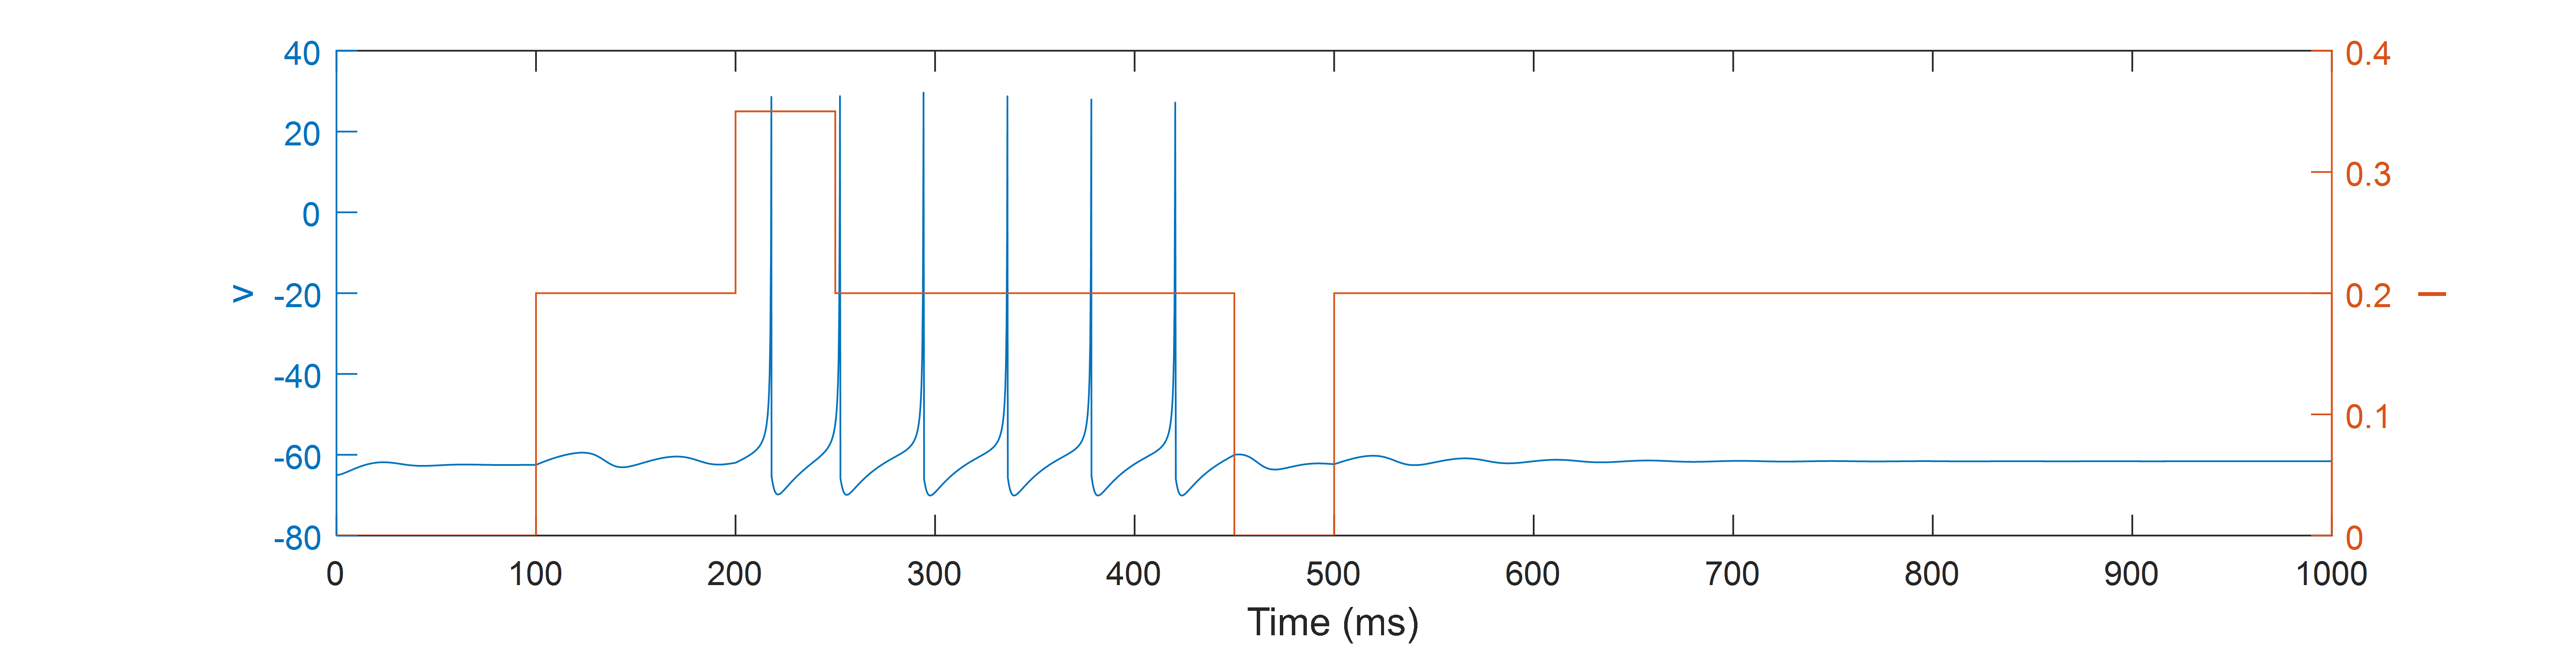
\includegraphics[width = 150mm, scale = 0.8]{./fig/experiment.png}
  \caption{The expected firing rate change in Izhikevich model when working memory is enabled.}
  \label{fig1}
\end{figure}

\bibliography{reference}{}
\bibliographystyle{abbrv}



\end{document}